\fixme{\bf This subsection should be checked for duplicated content in the APA chapter.}

\fixme{\bf The figure in this subsection should be updated to reflect the DUNE FD design.}

Each side of an APA includes four wire layers as described in Section~\ref{sec:fdsp-apa-design}. 
%The innermost X-plane layer of wires is nominally biased at +820~V, with each wire AC coupled 
%to one of the 128 charge amplifier circuits on the FEMB. The V-plane wire layer is effectively biased at zero volts, 
%with each wire directly connected to one of the charge amplifier circuits. The U-plane wire layer is nominally 
%biased at $-$370~V with each wire AC-coupled 
%to one of the 128 charge amplifier circuits. The outermost G-plane wire layer,
%which has no connection to the charge amplifier circuits, is biased at $-$665~V.
Electrons passing through the wire grid must drift unimpeded until they reach the X-plane 
collection layer. The nominal bias voltages are predicted to result in this electrically 
transparent configuration, and are given in Section~\ref{sec:fdsp-apa-design}. 

The filtering of wire-bias voltages and AC coupling of wire signals passing
onto the charge amplifier circuits is done on capacitance-resistance (CR) boards that plug in between the APA wire-board stacks and FEMBs.
Each CR board includes single R-C filters for the X- and U-plane wire-bias voltages. In addition, each board has 48 
pairs of bias resistors and AC coupling capacitors for X-plane wires, and 40 pairs for the U-plane wires. The coupling capacitors block DC while passing AC 
signals to the CE motherboards.  A schematic diagram of the protoDUNE-SP APA wire bias subsystem is illustrated in Figure~\ref{fig:CR-board}.

\begin{dunefigure}
[protoDUNE-SP APA wire bias schematic diagram, including the CR board.]
{fig:CR-board}
{protoDUNE-SP APA wire bias schematic diagram, including the CR board.}
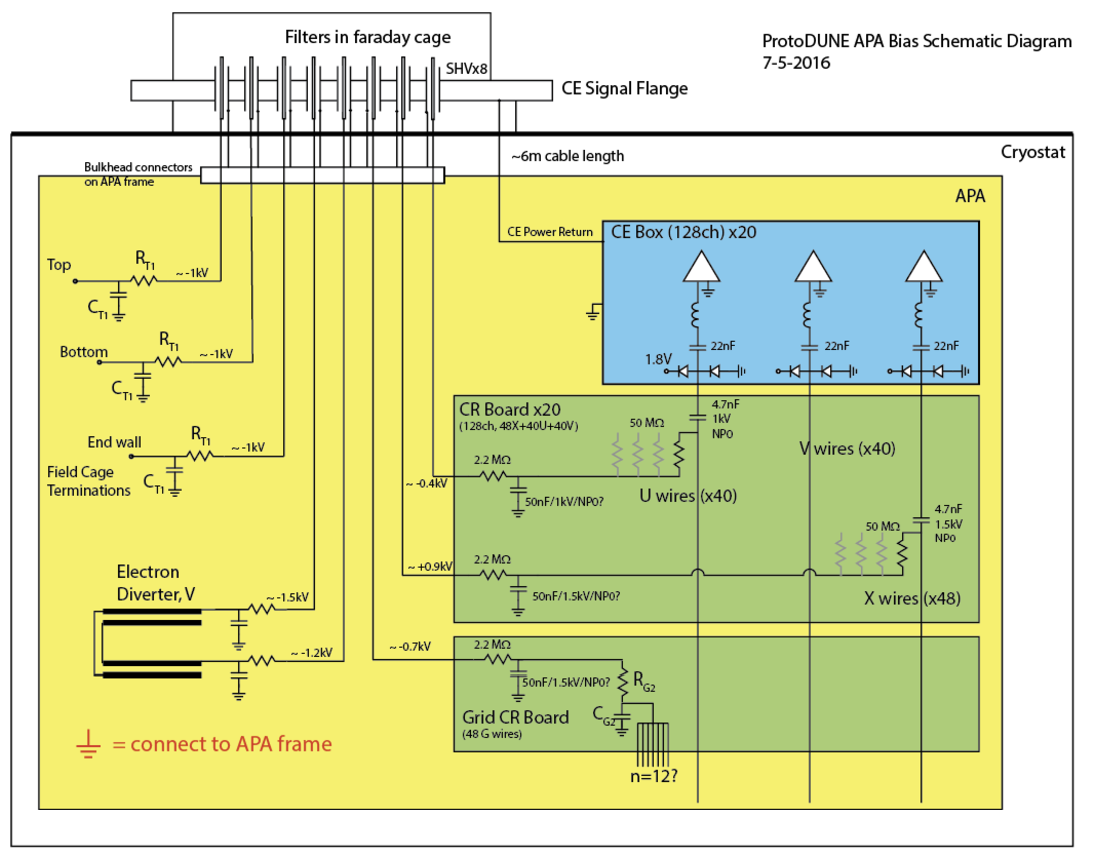
\includegraphics[width=0.8\linewidth]{tpcelec-cr_board.pdf}
\end{dunefigure}

%Separate CR boards include a single R-C filter for the G-plane wires and 12 pairs of bias resistors and
%coupling capacitors.
%Groups of four wires are tied together to share single
%bias resistors and filter capacitors. These CR boards do not connect to the charge amplifier circuits on the FEMB.

Clamping diodes limit the input voltage received at the amplifier circuits to between 1.8~V~$\pm$~U$\_$D, where U$\_$D
is the breakdown voltage of the diode $\sim$0.7~V.
The amplifier circuit has a 22~nF coupling capacitor at input to avoid leakage current from the protection clamping diodes. 

%%% UNCLEAR, REMOVE FOR NOW
%Coupling capacitors for the X-plane and U-plane wires are required to block DC bias voltages.
%However they also impact the efficiency of the detector circuits.
%The sense wires are expected to have $\sim200$~pF of capacitance to the APA frame.
%Induced or collected charges are effectively divided between the wire capacitance and the coupling capacitor.
%To achieve a charge-calibration accuracy of 0.5 percent or better,
%the coupling capacitors must be 4.7\,nF at ten percent tolerance, or 2.2\,nF at five percent tolerance.
%Voltage ratings should be at least 1.5 times the expected operating voltages.

Bias resistance values should be at least 20\,M$\Omega$ to maintain negligible noise contributions.
The higher value helps to achieve a longer time constant for the high-pass coupling networks.
Time constants should be at least 25 times the electron drift time so that the undershoot in the digitized waveform
is small and easily correctable.
However, leakage currents can develop on PC boards that are exposed to high voltages over extended periods.
If the bias resistors are much greater than 50\,M$\Omega$, leakage currents may affect the bias voltages applied to the wires. The target value of 50\,M$\Omega$ was used in protoDUNE-SP.

The bias-voltage filters are R-C low-pass networks.
Resistance values should be much smaller than the bias resistances to control crosstalk between wires
and limit the voltage drop if any of the wires becomes shorted to the APA frame.
The value of 2.2\,M$\Omega$ was used in protoDUNE-SP.
Smaller values may be considered for DUNE although a larger filter capacitor would be required to maintain a given level of noise reduction.
The target value of 47\,nF was used in protoDUNE-SP for the filter capacitors.

%For the grid-plane bias filters, component values are less critical.
%If possible they will be identical to those used for the bias resistors and coupling capacitors
%(50~M$\Omega$ and 2.2 to 4.7\,nF).
